\section{Ordine del giorno}
\begin{enumerate}
\item Discussione sulle tecnologie 
\item Pianificazione per prima revisione
\item Metodo Agile
\item Coordinamento interno 
\end{enumerate}

\subsection{Discussione sulle tecnologie}



\subsection{Pianificazione per prima revisione}
Il team a fronte della prima revisione RTB ha stilato una lista delle cose da fare procedendo all'indietro.Creando una lista delle cose da fare inserite poi all'interno di una linea temporale con data ultima quella della prima revisione.
Questa linea temporale verrà poi approfondita nella sezione successiva "\textit{Metodo Agile}".


\subsection{Metodo Agile}
Dato lo svolgimento del progetto il gruppo ha deciso di adottare un metodo di lavoro agile al fine di aumentare la produttività.
Si è optato per un modello SCRUM e in vista della prima revisione si sono previsti 3 periodi di sprint ciascuno di 2 settimane. 
Per ogni sprint si è pianificato il lavoro da fare in modo tale da non doverlo organizzare nel periodo stesso dello svolgimento.
Di seguito la figura rappresentante la linea temporale in vista della prima revisione e i tre sprint nello specifico. 
\begin{center}
	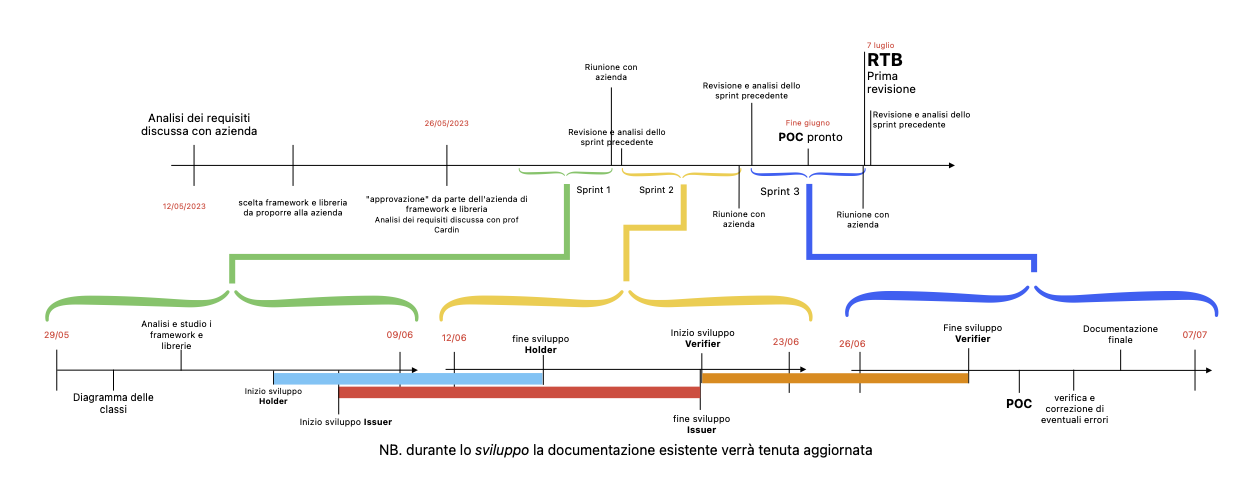
\includegraphics[scale = 0.35]{./res/images/RTB-1a-revisione.png}
\end{center}

\subsection{Coordinamento interno}
Si è fatto il punto della situazione sul lavoro effetuato durante la settimana corrente ed il gruppo si è sincronizzato e allineato; il responsabile inoltre ha suddiviso i ruoli e le mansioni da svolgere la settimana seguente. 
